\chapter{Decision Trees}
\section{Introduction}
Generally speaking, decision trees represent a certain type of graph known as trees, which are acyclic connected graphs. Details can be found in the mathematics branch graph theory; see for example, \cite{ref238, ref105}. Trees are commonly used in computer science and informatics for various purposes, to represent a hierarchical data structure, for example.

One of the popular traditional machine learning tools is a graph called rooted directed tree, in which the edges are directed from a node called root. An edge can point either to another (sub)tree or a node called leaf.

The path from the root to a leaf creates a branch. Every leaf is the terminal node of its path. A tree can generally be composed of any number of other trees that are called subtrees, thus modeling a hierarchy.

The properties of the rooted directed tree may be applied to creating models known as divide et impera (divide and rule), which is one of the reasons why these trees belong among the more popular machine learning algorithms for classification tasks. Another reason is that decision trees (if not excessively extensive) provide relatively understandable representation of knowledge, where a branch can also be taken as a rule. Leaves provide the answers to questions given by combinations of attribute values - in each node, there is a certain test for a specific value of an attribute and the tree branches from that node, each branch either to another node (subtree) on a lower level or to a terminal node called a leaf. If the tree method is used for classification, each leaf contains a label of a class. and the classified item receives its class according to specific combinations of attribute values, which are decided in the node.

Generally, to solve a problem, there can often be more than one alternative tree, and it is even possible that all such trees may provide the same result. Having several models available, an application should use the model with the lowest classification error. If there are trees with the same error (or without an error), then the simplest one is selected, following the practical Occam's razor rule: Simpler explanations are more likely to be correct; avoid unnecessary or improbable assumptions. A simpler tree means a tree with a lower number of nodes.

If a tree with a lower (zero) error is available, it must be used. Is there such a tree? A reader may try to create other possible trees (starting with different attribute tests in the tree root) to discover if there is one better than the suggested simple tree, which could be an interesting task.

In reality, it is not always possible to generate a tree that classifies with the zero error. The problem might be insufficient training data, non-linear boundaries between classes (a tree separates the problem space into subspaces using hyperplanes parallel with attribute axes), or something else.

In such a case, an application must settle for imperfection or look for a better solution by testing alternate algorithms. On the other hand, when a decision tree is a suitable solution for a given application and its data, the practice life prefers simpler solutions according to the Occam's razor rule. It means looking for the simplest possible tree which solves a given classification problem. In machine learning, several possible solutions have been found; for an example, see [36]. This chapter is going to deal with the very widely used tree-generating method known as c5-tree, which employs a concept for the minimization of trees called entropy minimization.

\section{Entropy Minimization-Based \texorpdfstring{$\boldsymbol{c}\mathbf{5}$}{c5} Algorithm}

In a nutshell, the entropy concept in informatics works with so-called chaos, which means that a set may have elements belonging to different classes. The goal is to split the set into subsets where each subset contains elements of just one class - then the entropy of such a subset is zero, or there is no chaos. The maximum entropy is in a set where mixed elements of various classes are evenly represented by the same number of their occurrence.

\subsection{The Principle of Generating Trees}
Sorting out such mixed up elements via entropy-minimization was the idea of John Ross Quinlan, who also wrote an interesting book which is a classic today, on the same \cite{ref220}. J. R. Quinlan is also an author of the first academic (and as well as commercial) successful implementation of his classification algorithm originally named ID3 (for discrete attributes) and later, after extending it for discrete and continuous attributes, missing attribute values, pruning, and some\\
other improvements, $c 4.5$ (one half of his book is a code in C ). In the course of time, this was continually modified, developing into an effective software tool now known as $c 5$; see also \cite{ref224}. $C 5$ is also available as a single-threaded version (not only) in R (GNU license) and its use is demonstrated in the text which follows.

Entropy is defined with the help of probabilities. It was introduced by one of the 'fathers' of informatics, Claude Elwood Shannon (1916-2001); for details, see [249]. According to Shannon, when there are two possibilities having probabilities, $p$ and $1-p$, the entropy, $H$, is defined as follows: Let $X$ be a discrete random variable that can take values from the set $\left\{x_{1}, x_{2}, \ldots, x_{n}\right\}$. Then $H(X)$ defines the entropy of $X$ this way:


\begin{equation*}
H(X)=-\sum_{i=1}^{n} p\left(x_{i}\right) \log _{2} p\left(x_{i}\right) \tag{7.1}
\end{equation*}


The logarithm base 2 is here because the information is measured in bits. To put it simply, at least $m_{b}$ bits are needed for $m$ registered cases stored in a set, so $m=2^{m_{b}}$, therefore $m_{b}=\log _{2}(m)$. If the probability, $p$, of selecting any case from the set is evenly distributed, then $p=1 / m$, therefore $m_{b}=\log _{2}(1 / p)= -l o g_{2}(p)$. In addition, the minus sign enables working with just positive numbers ( $0.0 \leq H(X) \leq 1.0$ ) because numerically negative information is neither defined nor used in informatics.

When a set is purely homogeneous, the probability of having elements of only one class is 1 and for other classes 0 . Thus, it is guaranteed that a randomly selected element from such a set belongs to a certain class with probability $p=$ 1 and, selecting an element from a different class has the probability $p=0$. Therefore, $p \cdot \log _{2} p=1 \cdot \log _{2} 1=0$, which is the minimum entropy, and (for two classes) if the ratio of elements in that set is $50 \%: 50 \%$, that is, $p=0.5$, then the entropy is maximum because $0 \cdot \log _{2} 0=1$ (after processing by L'Hôspital's rule). In other words, if the entropy is 0 , it is not necessary to investigate the contents of a set because the information about it is maximum.

The graph, Figure 7.1 illustrates the entropy curve shape expressing Eq. 7.1. Consider the horizontal axis $X$, a homogeneous set has the probability $p=0$ that it contains an element which does not belong to it - therefore, the entropy of that set is minimum, $H(X)=0$. Similarly, on the other end of the axis, $p=1$, that is, any selected element from that set belongs only to that set - the set is also quite homogeneous and its $H(X)=0$. If the set contains elements belonging to other sets, it is heterogeneous and the worse case is when $p=0.5$, or there is a mixture of 'own' and 'foreign' elements with the ratio $50 \%: 50 \%$ for two classes: $H(X)=1$, maximum entropy.

According to Quinlan's idea, a generated decision tree's task is not only to divide the original heterogeneous set into more homogeneous subsets but also reduce its size with respect to the number of nodes to as small as possible. Theoretically, it is possible to generate all possible trees and then choose the optimal
\begin{figure}[!ht]
\begin{center}
  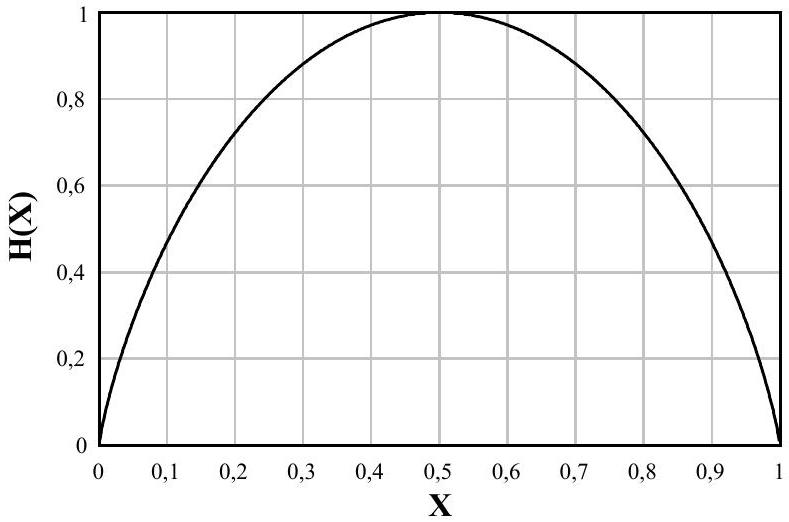
\includegraphics[width = 0.6\textwidth]{chapter/chapter7/2025_10_21_5ba6420d88ee7388cb5eg-191.jpg}
\caption{Entropy $H(X)$ curve shape.}
\end{center}
\end{figure}
one (lowest in error and size). Practically, however, it cannot be done because there may be too many trees and the computational complexity would be too high. In artificial intelligence, including machine learning, such cases can use some heuristics, while these do not guarantee optimal achievement, the result may be quite acceptable.

It should be noted here that the attributes of samples are supposed to be mutually independent - if the assumption is not fulfilled (which may for example, be due to significant correlation), the results may not be reliable. Therefore, attributes that depend on others should be discarded before processing. Such an assumption is, in machine learning, typical.

The $C 5$ tree generator successively tries one attribute after another to find which one decreases the entropy the most. Such an attribute $a_{i}$ is then selected as a node, which - in accordance with the results of testing its value - creates a new, hierarchically lower level in the tree, a subtree.

This tree node $a_{i}$ divides the heterogeneous set into more homogeneous subsets for the given training date set $T$ so that the eventual average entropy value of the resulting subsets maximally reduces the original entropy $H(T)$ of their parent set.

Therefore, the selected attribute $a_{i}$ provides the highest information gain $= H\left(T, a_{i}\right)=H(T)-H\left(T \mid a_{i}\right)-$ in other words, the maximal entropy difference, or decrease.

The average entropy is usually calculated using the following formula based on a posteriori probabilities and the individual entropies of newly formed leaves:


\begin{equation*}
H_{a v g}=\sum_{b} \frac{n_{b}}{n_{t}} \cdot(\text { chaos in a branch } b)=\sum_{b} \frac{n_{b}}{n_{t}} \cdot \sum_{c}\left(-\frac{n_{b . c}}{n_{b}} \log _{2} \frac{n_{b . c}}{n_{b}}\right), \tag{7.2}
\end{equation*}


where $n_{b}$ is the number of samples in a branch $b, n_{t}$ the number of samples in all branches leading from the splitting note, and $n_{b, c}$ the total number of all samples in the branch $b$ of a class $c$.

As a reader can see, the formula 7.2 calculates the average entropy of a subtree (created by dividing a heterogeneous set into more homogeneous subsets) by calculating the entropy for each subset (the second sum on the right side) and weighting it by the relative number of samples it covers (the first sum on the right side). Note this is not the only possible formula but it is, in practice, commonly used due to good results it obtains.

If it is not possible to further reduce the entropy, the tree generating process stops and the branches end in leaves. Otherwise, the whole process continues recursively, testing all attributes again and again. It cannot be excluded that such a tree is not theoretically optimal; practically, however, this method provides very good outputs and this is why it is so favored in research and applications.

To demonstrate the contribution of an attribute to the entropy decrease, let us take again a simple decision problem 'good/bad weather' demonstrated already in section 5.5 :

\begin{enumerate}
  \item it is nice weather $\oplus$
  \item it is cold $\ominus$
  \item it is not very cold $\oplus$
  \item not nice $\ominus$
  \item very cold
  \item cold $\ominus$
  \item very nice weather
\end{enumerate}

In the original set of training samples, members of both classes (three positive, pos, $\oplus$, and four negative, neg, $\ominus$ ) are mixed together, hence the chaos.

The entropy of this considerably heterogeneous set can be quantified using Eq. 7.1 as follows (recall that $0 \cdot \log _{b} 0=0$, and $\log _{b} x=\log _{10} x / \log _{10} b$, thus $\log _{2} x=\log _{10} x / \log _{10} 2$, or instead of $\log _{10} \log _{e}$ can be used as well):

$$
H(X)=-\frac{3}{7} \cdot \log _{2} \frac{3}{7}-\frac{4}{7} \cdot \log _{2} \frac{4}{7} \doteq 0.9853 .
$$

As it can be seen, the entropy is very high, close to 1.0 because the ratio of the number of members in both classes is $3 \oplus: 4 \ominus$. For example, using the attribute weather (with frequencies either 0 or 1 in a sample) for splitting the original set into two more homogeneous subsets, and taking the help of Eq. 7.2 for computing the average entropy $H_{\text {avg }}$ after splitting, a very simple decision tree generated by $c 5$ could look like the graph in Figure 7.2. The division assumes that if the word 'weather' is included, it is a positive case, otherwise a negative one.

This approach correctly covers two positive cases (No. 1 and 7); however, one case (No. 3) is classified incorrectly. All the negative cases are covered correctly.

\begin{figure}[!ht]
\begin{center}
  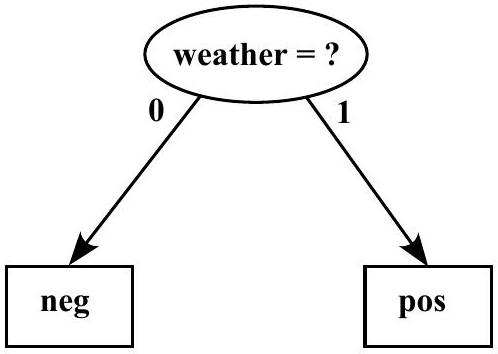
\includegraphics[width = 0.4\textwidth]{chapter/chapter7/2025_10_21_5ba6420d88ee7388cb5eg-193.jpg}
\caption{A decision tree solving the problem 'good/bad weather' with one error produced by the left branch ( $H>0$ ): without weather it is a negative message (one incorrect classification), otherwise a positive one (the right branch with $H=0$ ).}
\end{center}
\end{figure}

The contribution of weather to the entropy decrease may, therefore, be numerically calculated as follows:

$$
H_{\text {avg }}=\frac{5}{7} \cdot\left(-\frac{4}{5} \log _{2} \frac{4}{5}-\frac{1}{5} \log _{2} \frac{1}{5}\right)+\frac{2}{7} \cdot\left(-\frac{2}{2} \log _{2} \frac{2}{2}-\frac{0}{2} \log _{2} \frac{0}{2}\right) \doteq 0.5157 .
$$

The calculation computes the left branch entropy (which is $>0$ ) and the right branch entropy (which is $=0$ ) for each class, employing the respective a posteriori probabilities in the expressions $p \cdot \log _{2} p$ as well as the weights ( 5 cases for the left and 2 cases for the right branch out of 7).

Obviously, the initial entropy was significantly reduced and the not negligible information gain is $0.9853-0.5157=0.4696$. An interested reader may similarly compute the entropies, contributions of other attributes, and/or add some additional splitting to further decrease the chaos.

\subsection{Pruning}
The generated tree, without any further modifications, can simply serve as the exact model of the specific data from which it was created. However, if the tree is to be used for future classifications or predictions, it should represent the most general knowledge derived from the particular training data. In such a case, the so-called pruning process is used to improve the generalization of the obtained model. Pruning means the replacement of a subtree by a leaf, that is. a certain simplification of the tree.

From the point of view of training examples, this simplification may lead to a higher classification error related to training examples, which the unpruned tree can otherwise correctly classify into classes even optimally, with a zero error. Such a tree is so-called over-fitted, that is, it can properly classify mainly or only
the training examples and fails to correctly process others. However, the aim is to also best classify cases that are not (or cannot be) included in the training set.

Practice shows that some generalization of the tree by pruning can increase (sometimes significantly) the classification accuracy on future data at the cost of a modest reduction of the same for the training data. The tree pruning rate can be controlled by a parameter which indicates the maximum allowed reduction of the tree. Typically, it is limited to 25 percent but sometimes, it is worth experimentally finding an optimal value.

The idea of the pruning process is illustrated in Figure 7.3. On the left side, a subtree perfectly assigns classes (white and black points). The node $x_{j}$ has a left branch directed to a leaf covering five white cases, which is fairly general in comparison with the right-directing branch leading to a leaf covering only one, thus, too specific case - a black point.

Replacing the whole subtree $x_{j}$ (consisting of the node $x_{j}$ and its two leaves) with the left-sided leaf of $x_{i}$ (see the right side of the figure) containing five correct white and one incorrect black point slightly increases the classification error measured by the training samples. However, it may decrease the error measured by testing samples - the over-fitting is reduced in favor of generality.

As an example, let us consider two possible solutions of the weather problem discussed above (see Figure 7.2 and Figure 7.4). The weather-tree in Figure 7.2 says that if the word weather is present in a text example, the decision is pos: good weather; otherwise, neg: bad weather. According to the generated tree, no other word is necessary for the decision: no good, bad, nice, cold, etc. Is it a correct decision tree? Should it look like that? Can there be a better, more accurate tree? As for the correctness, the presented decision tree in Figure 7.2 makes one mistake because in the sample 3 (which is correctly pos) attribute weather is not present but the tree classifies it wrongly as neg. The remaining six samples are classified correctly, so the classification accuracy is approximately $85.7 \%$.

\begin{figure}[!ht]
\begin{center}
  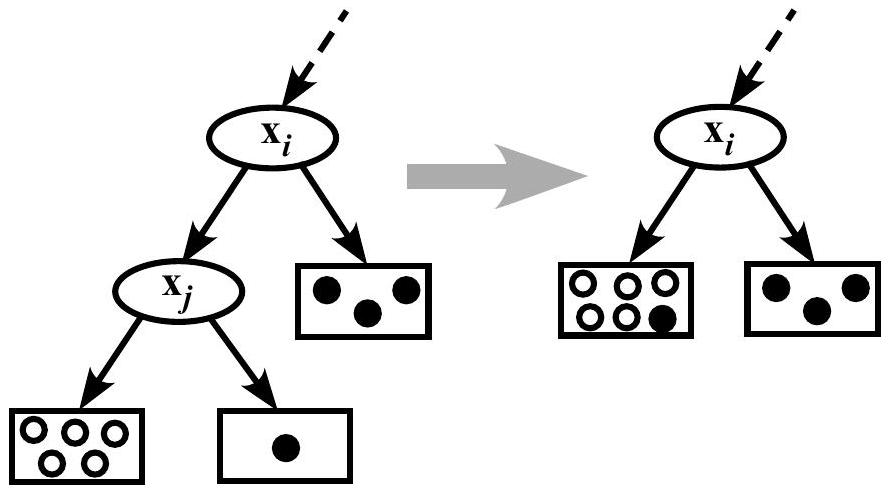
\includegraphics[width = 0.5\textwidth]{chapter/chapter7/2025_10_21_5ba6420d88ee7388cb5eg-194.jpg}
\caption{Replacing a subtree (on the left) with a leaf (on the right) by pruning.}
\end{center}
\end{figure}

\begin{figure}[!ht]
\begin{center}
  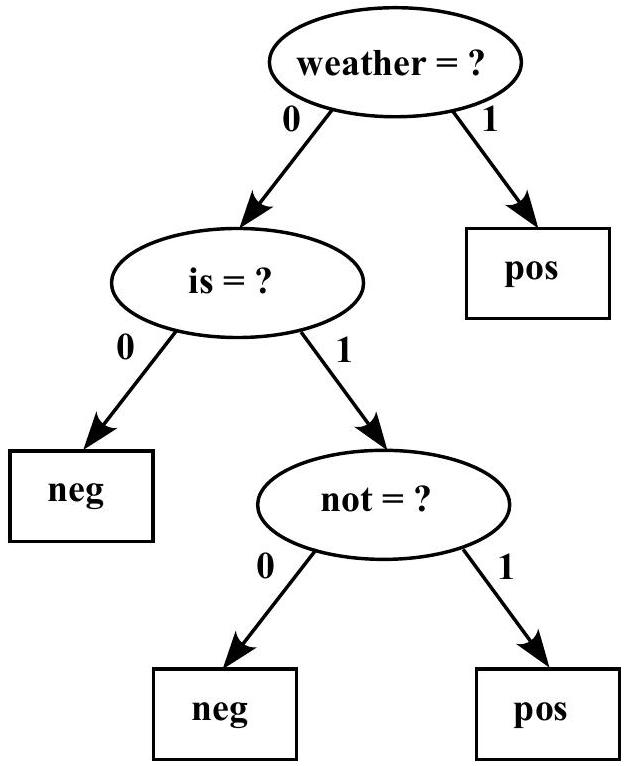
\includegraphics[width=0.5\textwidth]{chapter/chapter7/2025_10_21_5ba6420d88ee7388cb5eg-195.jpg}
\caption{A full-size, unpruned decision tree variant dealing perfectly with the content meaning problem of the weather phrases 'good/bad weather'.}
\end{center}
\end{figure}

As is apparent, the model is not quite perfect, but from the point of view of generality, could that one mistake be forgiven - or not? This can only be evaluated on the basis of testing, which was not done here because of the triviality of the artificial demonstration task and the absence of training samples.

Figure 7.4 shows an alternative tree for the same training data. However, this time it is a complete variant which classifies the training data perfectly, without that one error in the previous case as demonstrated in Figure 7.2. The tree in Figure 7.2 may represent the pruned tree shown in Figure 7.4, replacing two testing nodes and three leaves with just one leaf for the price of a single mistake. Again, it is not possible to assess the generality of both trees without testing. It is obvious, however, that (in view of the new circumstances) the tree in Figure 7.4 is more complex, testing values of three attributes (weather, is, not), not just one (weather).

From the application point of view, the question is, is it worthwhile to use the more complicated tree or just the simpler model? The answer must be sought by users themselves, based on the needs of the produced application including time and memory demands. Models in the real world are usually much more extensive and more complicated; thus, it is very important to test them as carefully as possible before they are put into practice.

\section{C5 Tree Generator in R}
Using the same dataset, BookReviews1000.csv, with samples of book reviews, this section presents a possible application of the $C 5$ tree classifier to text mining.

First, the creation of a decision tree is demonstrated. Second, the tree properties are briefly discussed, pointing out the acquired useful information. Third, how to assess the accuracy of tree classification is demonstrated so that it can be applied to future data. Finally, the ability of the tree to provide understandable knowledge in the form of rules is shown.

\subsection{Generating a Tree}
In the first demonstration, the first 100 samples serve as testing items while the remaining 900 are used for training. The source R-code, employing the C50 package, used for generating the $C 5$-tree including the corresponding testing rules and using both testing samples is as follows:

\begin{verbatim}
library(C50)
# loading the data
data <- read.csv("BookReviews.csv", header=TRUE)
# converting the data to a matrix
dtm <- as.matrix(data)
# removing the object data (unnecessary from now)
rm(data)
# number of instances
n <- dim(dtm)[1]
# number of attributes
m <- dim(dtm)[2]
# indexes of 100 testing samples
number_of_test_samples <- 100
test_index <- 1:number_of_test_samples
# selecting training samples
train_data <- dtm[-test_index, 1:(m-1)]
train_labels <- dtm[-test_index, m]
\end{verbatim}

\begin{verbatim}
# selecting testing samples
test_data <- dtm[test_index, 1:(m-1)]
test_labels <- dtm[test_index, m]
# training a c5 model (tree and rules)
c5_tree <- C5.0(train_data, as.factor(train_labels))
c5_rules <- C5.0(train_data, as.factor(train_labels),
    rules=TRUE)
# visualizing the generated decision tree
plot(c5_tree)
# printing the detailed summary for the generated
# decision tree and rules
print(summary(c5_tree))
print(summary(c5_rules))
# calculating class predictions for the tree
predictions <- predict(c5_tree, test_data, type="class")
# creating a confusion matrix
cm <- table(test_labels, predictions)
print("Confusion matrix")
print(cm)
# number of instances
n <- sum(cm)
# number of correctly classified instances for each class
correct <- diag(cm)
# numbers of instances in each class
instances_in_classes <- apply(cm, 1, sum)
# numbers of each class predictions
class_predictions <- apply(cm, 2, sum)
# accuracy
accuracy <- sum(correct)/n
# precision per class
precision <- correct/class_predictions
\end{verbatim}

\begin{verbatim}
# recall per class
recall <- correct/instances_in_classes
# F1-measure per class
f1 <- 2 * precision * recall / (precision + recall)
# printing summary information for all classes
df <- data.frame(precision, recall, f1)
print("Detailed classification metrics")
print(df)
print(paste("Accuracy:", accuracy))
# macroaveraging
print("Macro-averaged metrics")
print(colMeans(df))
# microaveraging
print("Micro-averaged metrics")
print(apply(df, 2, function (x)
    weighted.mean(x, w=instances_in_classes)))
\end{verbatim}

The $C 5$ tool generates a tree model according to the training samples. The tree is then displayed together with the result describing the classification of training samples. The console output is a result in a text-like form, where the positive class is marked as 1 and the negative one as 0 . The tree is not trivial, so it is divided between several parts (subtrees). Due to the tree size, it is not copied here in total, just the root and a couple of levels under it have been shown:

\begin{verbatim}
Call:
C5.O.default(x = train_data, y = as.factor(train_labels))
C5.0 [Release 2.07 GPL Edition] Tue Feb 19 09:03:50 2019
Class specified by attribute 'outcome'
Read 900 cases (2218 attributes) from undefined.data
Decision tree:
waste > 0:
\end{verbatim}

\begin{verbatim}
:...more <= 1: 0 (40)
: more > 1: 1 (3/1)
waste <= 0:
:...boring > 0:
    :...day <= 0: 0 (49/1)
    : day > 0: 1 (4/1)
    boring <= 0:
    :...tale > 0:
        :...apparently <= 0: 1 (25/1)
        : apparently > 0: 0 (3/1)
        tale <= 0:
\end{verbatim}

The rest of this tree (after the branch tale <= 0 ) has been left out. Its graphical depiction is shown in Figure 7.5 (again, only the top of the tree).

\begin{figure}[!ht]
\begin{center}
  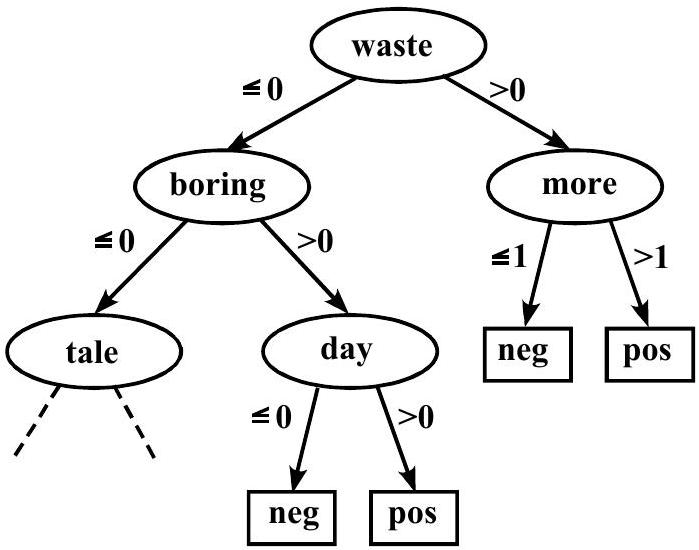
\includegraphics[width=0.5\textwidth]{chapter/chapter7/2025_10_21_5ba6420d88ee7388cb5eg-199.jpg}
\caption{The generated C5-tree (only its beginning and the root attribute waste are shown here).}
\end{center}
\end{figure}

\subsection{Information Acquired from C5-Tree}
The word waste is present in the root. From the entropy minimization point of view, it is the best attribute and each classification starts with a test checking whether the numeric representation of this word (in this case, its frequency in a document) is $>0$ or $\leq 0$ (however, frequency cannot be $<0$ ).

After dividing the documents (the original set) between two categories (subsets) with and without waste, the entropy can be further reduced because, on the next level, the word more again divides documents (those without waste) between two categories. This branch ends because further lowering of the entropy is not possible here.

The branch leading to the class 0 covers exactly 40 documents having the frequency of the word more $\leq 1$, while the other branch covers 4 documents containing more having its frequency $>1$; however, one of them is classified incorrectly (in the $C 5$ output, it is indicated by $3 / 1$, or 3 correctly classified and 1 incorrectly).

Documents without waste can be further divided into the category with boring and without boring, and then again using tale and day, and so on. Documents having no boring but with the attribute tale may be further divided to reduce the entropy, which is not illustrated at this point (but can be seen in the complete computational output), while the word day finishes a branch: without day, the classification is 0 (negative) for $49 / 1$ cases, otherwise 1 (positive) for $4 / 1$. Individual branches make rules together; for example, if waste $=0 \wedge$ boring $> 0 \wedge$ day $>0$ then positive.

In the textual tree representation below, the summary says that the tree size is 108 nodes. From the classification point of view, the accuracy error measured on training data is $4.9 \%$, that is 44 from 900 samples. In addition, the appended confusion matrix shows how many negative samples (marked as 0 ) were classified correctly (425) and incorrectly (18). Similarly for the positive samples: 431 correctly, 26 incorrectly. There are, altogether, ( $18+26$ ) - 44 incorrect classifications. Optimally, the confusion matrix should contain only non-zero numbers in its main diagonal (everything correctly classified) while the minor diagonals should contain only zeros (for any number of classes):

Evaluation on training data (900 cases):

\begin{flushleft}
\begin{tabular}{lrl}
\multicolumn{3}{c}{Decision Tree} \\
\cline { 1 - 2 }
Size & Errors &  \\
108 & $44(4.9 \%)$ & $\ll$ \\
 &  &  \\
\begin{tabular}{rrl}
(a) & (b) & $<$-classified as \\
--- & --- &  \\
\end{tabular} &  &  \\
\hspace{0.2cm}425\hspace{0.45cm}18\hspace{0.5cm}(a) : class 0 \\
\hspace{0.2cm}26\hspace{0.55cm}431\hspace{0.4cm}(b) : class 1 \\
\end{tabular}
\end{flushleft}

From the text-mining point of view, the generated tree also provides valuable information concerning so-called relevant attributes. The relevancy here means how much an attribute contributes to entropy reduction, that is, revealing what is typically common for each class - which words or phrases. A relevant attribute efficiently separates cases belonging to different classes. A list of relevant attributes is available (under Attribute usage heading) in the tree generator output. The attributes are ordered according to the number (in percentage) of times they are used for classification. An attribute in the tree root is tested every time ( $100 \%$ ). Attributes on lower levels are used less and less. Many attributes (often a very large majority) are never used, thus they are insignificant from the classification point of view; here, it is only 96 from 2218 , or $4.33 \%$. In the experiment presented, the tree gives such a list of relevant attributes; see Figure 7.6.

The activity of the relevant attributes on different tree levels can be studied in the complete computational output; for example, which values are used for branching or how significant they are.

\begin{figure}[!ht]
    \centering
    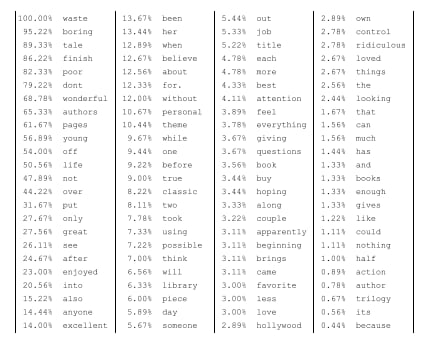
\includegraphics[width=\textwidth]{chapter/chapter7/figure7.6.jpg}
    \caption{The list of 96 relevant attributes generated by the 55 decision tree. The attributes are
ordered according to their frequency of their use. 100% (waste) in the root is the input attribute
tested always.}
    \label{fig:placeholder71}
\end{figure}

\subsection{Using Testing Samples to Assess Tree Accuracy}
The low classification error, $4.9 \%$, indicates that the tree-model itself is very good, with a high accuracy $95.1 \%$. If the goal is to create a model based on just the available data, without the intention to use it for the classification/prediction applied to new data in the future, a data/text miner might be fully satisfied. On the other hand, such a model represents only data from the past and can be strongly tied to the used training dataset - overtrained, without sufficient generalization that could be applied to unseen data items, whether from the past or the future.

This is the reason why the expected classification accuracy for the future data must be estimated using a disjunctive set of samples - testing samples. In the R-code above, the initial 100 samples were used for testing because those items were not used for training. The model created with the mentioned 900 training samples gives the following output on RStudio console:

[1] "Confusion matrix"\\knn\_mode

\begin{flushleft}
\begin{tabular}{lll}
test\_labels & 0 & 1 \\
0 & 36 & 21 \\
1 & 14 & 29 \\
\end{tabular}
\end{flushleft}
\begin{verbatim}
[1] "Detailed classification metrics"
    precision recall f1
0 0.72 0.6315789 0.6728972
1 0.58 0.6744186 0.6236559
[1] "Accuracy: 0.65"
[1] "Macro-averaged metrics"
precision recall f1
0.6500000 0.6529988 0.6482766
[1] "Micro-averaged metrics"
precision recall f1
0.6598000 0.6500000 0.6517234
\end{verbatim}

In this case, the accuracy is appreciable lower, just $65 \%$. Both positive and negative review samples have a very similar precision, $65 \%$ and $72 \%$, respectively. The overall error, $35 \%$, is relatively high, indicating that the model is not very good for the classification of unseen data.

A possible explanation might be that the training samples did not sufficiently cover the investigated area because only 900 reviews related to various book topics was not enough. It is likely the main reason as there are thousands of topics and millions of book readers.

A remedy for this situation could be to collect larger training data in subsets, which would cover more specific topics. Then, a model for each such subset could be generated, creating not only one universal classifier but a set of 'experts' for individual topics - which is how people do it. In any case, such situations need careful analysis. An alternative approach might also be to try several different classification algorithms in the hope that one of them would provide better results for a given application.

\subsection{Using Cross-Validation to Assess Tree Accuracy}
Secondly, the testing process applies the 10 -fold cross-validation method. The code is not presented here, since it is identical to the cross-validation code in Chapter 5, except for two rows, creating and using a decision tree model instead of a probabilistic model. The results for each of 10 computation steps as well as for the final summarizing step that provides the overall accuracy are available on Console:

\begin{verbatim}
Cross-validation fold: 1
    Accuracy: 0.65
    Precision(positive): 0.58
    Precision(negative): 0.72
Cross-validation fold: 2
    Accuracy: 0.74
    Precision(positive): 0.76
    Precision(negative): 0.72
Cross-validation fold: 3
    Accuracy: 0.62
    Precision(positive): 0.6530612
    Precision(negative): 0.5882353
Cross-validation fold: 4
    Accuracy: 0.63
    Precision(positive): 0.5849057
    Precision(negative): 0.6808511
Cross-validation fold: 5
    Accuracy: 0.63
    Precision(positive): 0.6346154
    Precision(negative): 0.625
Cross-validation fold: 6
    Accuracy: 0.64
    Precision(positive): 0.6808511
    Precision(negative): 0.6037736
\end{verbatim}

\begin{verbatim}
Cross-validation fold: 7
    Accuracy: 0.58
    Precision(positive): 0.4901961
    Precision(negative): 0.6734694
Cross-validation fold: 8
    Accuracy: 0.59
    Precision(positive): 0.62
    Precision(negative): 0.56
Cross-validation fold: 9
    Accuracy: 0.53
    Precision(positive): 0.537037
    Precision(negative): 0.5217391
Cross-validation fold: 10
    Accuracy: 0.74
    Precision(positive): 0.7818182
    Precision(negative): 0.6888889
Average Accuracy: 63.5 %
SEM: 2.07
\end{verbatim}

Apparently, the result is very similar to the testing with 100 external samples. It confirms also, the mean error value $=63.5 \%$, as well as a low standard error of the mean, SEM = 2.07, which evidences that there is small dispersion of results for each of ten steps. Therefore, the model is stable; however, its classification accuracy is not very good.

The conclusion can be the same as in the case with the external 100 testing samples briefly discussed above.

\subsection{Generating Decision Rules}
Decision rules, having the format IF-THEN, are generally favored because they represent relatively easily understandable knowledge, and if there is a 'reasonably' sized set of rules (for example, ten), their application is preferred - provided that the rules work well with high accuracy, given their application area. Rules can also be used, for example, for filling up a knowledge base.

The principle of generating rules consists of taking individual tree branches from the root to leaves; each branch may represent a rule. This procedure can also involve certain optimization like removing redundant rules; for example, in the case of the rules IF $x_{1}$ THEN $y$ and IF $x_{1} \wedge x_{2}$ THEN $y$, only the first rule suffices.

The $C 5$-tree generator was applied to the demonstration data and the task was to create an adequate set of rules. In all, 20 rules were generated and the output shows them all. Only the first two (as copied from the output) are shown here for the purpose of illustration. Each rule represents a standard conjunction where attributes are tested for their frequency like in the tree nodes, and a leaf is on the right side of a rule. The transcription of the first rule into a more compact form looks like this (dont comes from don't, class 0 is negative):

IF before $\leq 0 \wedge$ classic $\leq 0 \wedge$ dont $>0 \wedge$ finish $\leq 0 \wedge$ not $>0 \wedge$ possible $\leq 0 \wedge$ put $\leq 0 \wedge$ theme $\leq 0 \wedge$ took $\leq 0$ THEN class $=0$

A piece of the $c 5$ output:

\begin{verbatim}
Rules:
Rule 1: (44, lift 2.0)
    before <= 0
    classic <= 0
    dont > 0
    finish <= 0
    not > 0
    possible <= 0
    put <= 0
    theme <= 0
    took <= 0
    -> class 0 [0.978]
Rule 2: (26, lift 2.0)
    along <= 0
    authors > 0
    best <= 0
    brings <= 0
    dont <= 0
    giving <= 0
    own <= 0
    wonderful <= 0
    -> class 0 [0.964]
\end{verbatim}

In the first rule, ( 44, lift 2.0 ) means 44 covered samples without an error (otherwise it is the same as for trees, $N / M$, where $N$ is the number of correctly classified training cases and $M$ the number of incorrectly classified ones by a rule). The lift 2.0 is the result of dividing the rule's estimated accuracy by the relative frequency of the predicted class in the training set.

The class assignment, -> class 0 [0.978], contains a value between 0 and 1 that indicates the confidence with which this prediction is made. If a case is not covered by any rule, then it is used as a so-called default class which, in this example, is Default class: 1 ( 1 means positive; can be found in the output).

After the list of rules, the output contains an evaluation of the rule set accuracy as well as a list of relevant attributes, as is done for trees. For example:

Evaluation on training data (900 cases):

Rules

No Errors

20 121(13.4\%) <<

\begin{flushleft}
\begin{tabular}{rrl}
(a) & (b) & <-classified as \\
\hline
358 & 85 & (a) : class 0 \\
36 & 421 & (b) : class 1 \\
\end{tabular}
\end{flushleft}

Attribute usage:\\
100.00\% waste\\
84.00\% life\\
30.67\% tale\\
25.89\% pages\\
$24.78 \%$ not\\
$22.56 \%$ dont\\
$21.44 \%$ wonderful\\
...

To obtain the result of testing the generated rules with 100 external samples, the same procedure as followed for the tree needs to be carried out. It is necessary to get class labels using the created model and test data:
\begin{verbatim}
    predictions <- predict(c5\_rules, test\_data, type="class")
\end{verbatim}
The rest of the calculations are the same as in the case of using a decision tree. The results of testing are shown here:\\[0pt]
[1] "Confusion matrix"
\begin{flushleft}
\begin{tabular}{lll}
test\_labels & 0 & 1 \\
0 & 32 & 25 \\
1 & 11 & 32 \\
\end{tabular}
\end{flushleft}

\begin{verbatim}
[1] "Detailed classification metrics"
    precision recall f1
0 0.7441860 0.5614035 0.64
1 0.5614035 0.7441860 0.64
[1] "Accuracy: 0.64"
[1] "Macro-averaged metrics"
precision recall f1
0.6527948 0.6527948 0.6400000
[1] "Micro-averaged metrics"
precision recall f1
0.6655896 0.6400000 0.6400000
\end{verbatim}

Again, it is obvious that testing samples give a higher accuracy error, $36 \%$, while the training samples are better with an error of only $13,4 \%$. However, the discussion about the tree is valid also for the rules - trees and rules are just two different representations of knowledge revealed from data.

The not quite convincing classification results in the demonstration presented above do not mean that decision tree or rules are inferior algorithms. There are a huge number of successful applications based on trees and rules, including text mining. The practice shows that varied data may need different algorithms and no algorithm is universal \cite{ref282} - what works for certain datasets does not have to be convenient for others and vice versa. Sometimes, a user has to select a less perfect algorithm just because it has significantly lower computational complexity and can be used in real time. On that account, machine learning is an open field for experimenting.